\documentclass[11pt]{amsart}


\usepackage{geometry}                % See geometry.pdf to learn the layout options. There are lots.
\geometry{a4paper}                   % ... or a4paper or a5paper or ...
%\geometry{landscape}                % Activate for for rotated page geometry
\usepackage[parfill]{parskip}    % Activate to begin paragraphs with an empty line rather than an indent
\usepackage{enumitem}
\usepackage{graphicx}
\usepackage{amssymb}
\usepackage{amsmath}
\usepackage{cancel}
\usepackage{tikz}
\usepackage{epstopdf}
\DeclareGraphicsRule{.tif}{png}{.png}{`convert #1 `dirname #1`/`basename #1 .tif`.png}
\usepackage{breqn}

\usetikzlibrary{calc,intersections,through,backgrounds,arrows,decorations.markings}

\tikzset{
  coordsys/.pic={
    \draw[->] (0,0) -- ++(6mm,0pt);
    \draw[->] (0,0) -- ++(0pt,6mm);
  },
  myarr/.style={decoration={
      markings,
      mark=between positions 0 and 1 step 2mm with {\arrow{stealth}},
    },
    postaction=decorate
  },
}

\title{Econ 210C Problem Set \# 3}
\author{Nathaniel Bechhofer}
%\date{}                                           % Activate to display a given date or no date

\begin{document}
\maketitle


\section{Variable labor supply in the RBC model}
\begin{figure}[h]
	\centering
	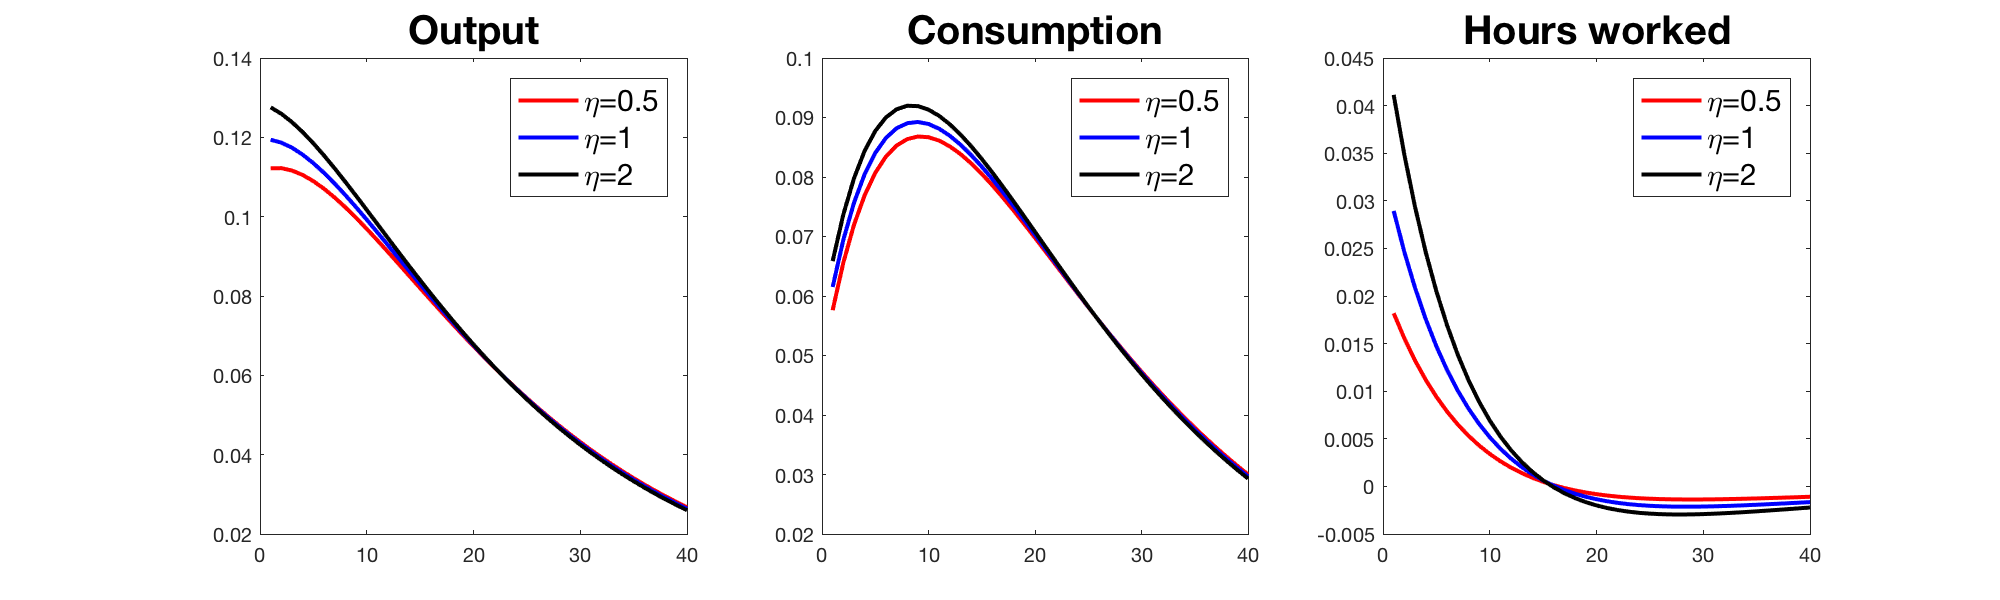
\includegraphics[width=\textwidth]{Minki/Q1}
	\caption{Impulse responses with varying $\eta$}
\end{figure}

\begin{table}[h]
	\centering
	\begin{tabular}{ccccc}
		\hline \hline 
		& $\eta=0.5$  & $\eta = 1$          & $\eta = 2$ & Data  \\
		\hline 
		$\sigma_Y$ &  1.54    & 1.64    & 1.74    & 1.72     \\
		$\sigma_C$ &  0.97    & 1.02   & 1.08       & 1.27 \\
		$\sigma_L$ &   0.23   &  0.37   & 0.53     &  1.59 \\
		\hline
	\end{tabular}
	\caption{Response to a transitory discount factor shock}
\end{table}
Larger Frisch elasticity values imply a better fit, as they generate stronger inter-temporal substitution of labor supply, amplifying the effect of shocks. 
Consumption is still too smooth, and the volatility of hours is too low. 

\newpage

\section{Variable capital utilization in an RBC model}

\subsection*{(a)}

Firms choose capital utilization $U$, capital $K$, and labor demand $N$.

The production function that we can use directly (since the output is the numeraire) is
\[
Y_t = (U_t K_{t-1})^{\alpha} (Z_t N_t)^{1-\alpha}
\]
and since the firms own capital, they face the constraint
\[
K_t = I_t + (1 - \delta(U_t)) K_{t-1}
\]
but they also have to pay wages $W_t N_t$ and invest $I_t$
so we can set up the Lagrangian
\begin{tiny}
\[
\mathcal{L} = E \sum_s (\prod_{k=1}^s (1+r_{t+k})^{-1}) \bigg{(} (U_{t+s} K_{t+s-1})^{\alpha} (Z_{t+s} N_{t+s})^{1-\alpha} - W_{t+s} N_{t+s} - I_{t+s} + q_{t+s} (-K_{t+s} +  I_{t+s} + (1 - \delta(U_{t+s})) K_{t+s-1}) \bigg{)}
\]
\end{tiny}
so we have first order conditions:

for labor we have
\[
W_t = (1-\alpha) (U_{t} K_{t-1})^{\alpha} Z_{t}^{1-\alpha} N_t^{-\alpha}
\]
for investment we have
\[
q_t = 1
\]
for capital at time $t$ we have
\[
q_t = E \left[ \frac{1}{1+r_{t+1}} \left( \alpha U_{t+1}^{\alpha} K_t^{\alpha -1} (Z_{t+1} N_{t+1})^{1-\alpha} + q_{t+1} (1 - \delta(U_{t+1})  \right) \right]
\]
and finally we have the condition for utilization
\[
\alpha U_t^{\alpha - 1} K_{t-1}^{\alpha} (Z_{t} N_{t})^{1-\alpha} = q_t K_{t-1} \delta'(U_t)
\]

Combining the investment and capital optimality conditions yields the expression for the rental rate of capital. 
\[
	R_{t+1} = \alpha U_{t+1}^{\alpha} K_t^{\alpha -1} \left(Z_{t+1} N_{t+1}  \right)^{1-\alpha} - \delta(U_{t+1})
\]
The rental rate depends on utilization because the marginal product of capital and its depreciation rate depend on utilization. 

\subsection*{(b)}
The log linearized version of the utilization optimality condition
	 \[
	 q_t \delta^{'}(U_t) K_{t-1}  = \alpha U_t^{\alpha -1} K_{t-1}^\alpha \left( Z_t N_t \right)^{1-\alpha}
	 \] 
	 is
	\begin{align*}
	&\check{q_t}+ \frac{\delta^{''}(\bar{U}) \bar{U}}{\delta^{'}(\bar{U})} \check{U}_t + \check{K}_{t-1} = (\alpha -1) \check{U_t} + \alpha \check{K_{t-1}}  + (1-\alpha) \left(  \check{Z_t} + \check{N_t}\right) 
	\end{align*}
We know $\check{q_t}=0$ from the investment optimality condition and  we also know 
\[
\check{Y_t} = \alpha \left( \check{U_t} + \check{K_{t-1}} \right) + (1-\alpha) \left(  \check{Z_t} + \check{N_t}\right)
\] 
because the production function is given, so we have
	\begin{align*}
	\check{U_t} = \frac{1}{1 + \Delta} \left( \check{Y_t} - \check{K_{t-1}}\right)
	\end{align*}

\subsection*{(c)}

The log-linearized production function is
	\begin{align*}
	\check{Y_t} &= \alpha \left( \check{U_t} + \check{K_{t-1}} \right) + (1-\alpha) \left(  \check{Z_t} + \check{N_t}\right) \\
	& = \frac{\alpha}{1 + \Delta} \left( \check{Y_t} - \check{K_{t-1}} \right) + \alpha \check{K_{t-1}} + (1-\alpha ) \left(  \check{Z_t} + \check{N_t}\right)
	\end{align*} 
	Isolate $\check{Y_t}$:
	\begin{align*}
	\check{Y_t} &= \frac{\Delta \alpha }{1 + \Delta - \alpha} \check{K_{t-1}} + \frac{(1+\Delta)(1-\alpha)}{1+ \Delta - \alpha} \left(  \check{Z_t} + \check{N_t} \right)  \\
	& = \check{Z_t} + \check{N_t} \quad \left( \text{when } \Delta = 0 \right) \\
	& = \alpha \check{K_{t-1}} + (1-\alpha) \left( \check{Z_t } + \check{N_t} \right)   \quad \left( \text{when } \Delta = \infty \right)
	\end{align*}

     $\Delta = 0$ implies the capital stock is impotent, and output thus only depends on technology and labor. 
$\Delta = \infty$ implies full utilization, so output depends on all three inputs, with weights equal to the Cobb-Douglas coefficients. 
    
In every other case, we have 
    \begin{equation*}
    \check{Y_t} = \frac{\Delta \alpha }{1 + \Delta - \alpha} \check{K_{t-1}} + (1-\alpha) \left( \check{Z_t} + \check{N_t} \right)+ \frac{\alpha (1-\alpha)}{1+ \Delta - \alpha} \left(  \check{Z_t} + \check{N_t} \right)
    \end{equation*}
    so $Z_t$ and $N_t$ in $Y_t$ matter relatively more (with capital not being fully utilized) relative to the $\Delta = \infty$ case. 


\section{Homework in macroeconomics}

\subsection*{(a)}

 The Lagrangian for the household's maximization problem is:
\[
	\mathcal{L} = \left( C_m^\rho + C_h^\rho \right)^{\frac{1}{\rho}} - \left( \frac{1}{\eta} + 1 \right)^{-1} \left(  L_h + L_m \right)^{\frac{1}{\eta} + 1} + \lambda \left( W L_m - C_m \right) + \xi \left(L_h - C_h \right)
\]
	The first order conditions for the interior solutions are:
	\begin{align*}
	\cancel{\frac{1}{\rho}}\left( C_m^\rho + C_h^\rho \right)^{\frac{1}{\rho} -1} \cancel{\rho}  C_m^{\rho-1} &= \lambda \\
	\cancel{\frac{1}{\rho}} \left( C_m^\rho + C_h^\rho \right)^{\frac{1}{\rho} -1} \cancel{\rho} C_h^{\rho-1} & = \xi \\
	\left(  L_h + L_m \right)^{\frac{1}{\eta} }  &=\lambda W \\
	\left(  L_h + L_m \right)^{\frac{1}{\eta} }  &= \xi 	 
	\end{align*}

\subsection*{(b)}

From the two first order conditions for labor, we have 
\[
\xi = \lambda W
\]

\subsection*{(c)}

From the two first order conditions for consumption, we have
\[
\xi = \lambda \left( \frac{C_h}{C_m} \right)^{\rho-1}
\]

\subsection*{(d)}

With the budget constraints binding, we have
\[
C_h = L_h
\]
and from above we get
\[
C_h = C_m W^{\frac{1}{\rho-1}}
\]

\subsection*{(e)}

We now have
\[
L_h = C_m W^{\frac{1}{\rho-1}}
\]
and we can assume the budget constraint holds for formal markets to make the substitution
\[
C_m = WL_m
\]
getting us
\[
L_h = WL_m W^{\frac{1}{\rho-1}}
\]
equivalent to
\[
L_h = L_m W^{\frac{\rho}{\rho-1}}
\]
and from our first order conditions we have
\[
L_h + L_m = (\lambda W)^{\eta}
\]
so we can substitute for $L_h$ to get
\[
(\lambda W)^{\eta} - L_m = L_m W^{\frac{\rho}{\rho-1}}
\]
so we have
\[
L_m (1 + W^{\frac{\rho}{\rho-1}}) = (\lambda W)^{\eta}
\]
and thus
\[
L_m = \frac{(\lambda W)^{\eta}}{(1 + W^{\frac{\rho}{\rho-1}})}
\]

\subsection*{(f)}

We now have
\[
\frac{\partial L_h}{\partial W} = \frac{(1 + W^{\frac{\rho}{\rho-1}}) \lambda^{\eta} \eta W^{\eta - 1} - (\lambda W)^{\eta} (\frac{\rho}{\rho-1}) W^{\frac{\rho}{\rho-1} - 1}}{(1 + W^{\frac{\rho}{\rho-1}})^2}
\]
with 
\[
\frac{\partial L_m}{\partial W} \cdot \frac{W}{L_m} = \frac{(1 + W^{\frac{\rho}{\rho-1}}) \eta  -  (\frac{\rho}{\rho-1}) W^{\frac{\rho}{\rho-1}}}{(1 + W^{\frac{\rho}{\rho-1}})}
\]
as the elasticity of $L_h$ with respect to $W$.

\subsection*{(g)}


\subsection*{(h)}

We had
\[
\left( C_m^\rho + C_h^\rho \right)^{\frac{1}{\rho} -1}  C_m^{\rho-1} = \lambda
\]
so substitute the budget constraints
\[
((W L_m)^{\rho} + L_h^{\rho})^{\frac{1}{\rho} -1} (W L_m)^{\rho-1} = \lambda
\]
and use the substitution
\[
L_h = L_m W^{\frac{\rho}{\rho-1}}
\]
to get
\[
((W L_m)^{\rho} + ( W^{\frac{\rho^2}{\rho-1}}) L_m^{\rho})^{\frac{1}{\rho} -1} (W L_m)^{\rho-1} = \lambda
\]
so now substitute back in to
\[
L_m = \frac{(\lambda W)^{\eta}}{(1 + W^{\frac{\rho}{\rho-1}})}
\]
and we have
\[
L_m = \frac{ \left[((W L_m)^{\rho} + ( W^{\frac{\rho^2}{\rho-1}}) L_m^{\rho})^{\frac{1}{\rho} -1} (W L_m)^{\rho-1}\right]^{\eta} W^{\eta}}{(1 + W^{\frac{\rho}{\rho-1}})}
\]
and we can simplify to get
\[
L_m = \frac{ \left[((W^{\rho} + W^{\frac{\rho^2}{\rho-1}}) L_m^{\rho})^{\frac{1}{\rho} -1} (W L_m)^{\rho-1}\right]^{\eta} W^{\eta}}{(1 + W^{\frac{\rho}{\rho-1}})}
\]
and again to get
\[
L_m = \frac{ \left[(W^{\rho} + W^{\frac{\rho^2}{\rho-1}})^{\frac{1}{\rho} -1} L_m^{1-\rho} (W L_m)^{\rho-1}\right]^{\eta} W^{\eta}}{(1 + W^{\frac{\rho}{\rho-1}})}
\]
and the $L_m$ terms on the right side cancel so we have
\[
L_m = \frac{ \left[(W^{\rho} + W^{\frac{\rho^2}{\rho-1}})^{\frac{1}{\rho} -1}  W ^{\rho-1}\right]^{\eta} W^{\eta}}{(1 + W^{\frac{\rho}{\rho-1}})}
\]
and we can rewrite the numerator to get
\[
L_m = \frac{ \left[(W^{\rho} + W^{\frac{\rho^2}{\rho-1}})^{\frac{1}{\rho} -1}  W ^{\rho}\right]^{\eta} }{(1 + W^{\frac{\rho}{\rho-1}})}
\] 
equivalent to 
\[
L_m = \frac{ \left[(W^{\rho}(1 + W^{\frac{\rho}{\rho-1}}))^{\frac{1}{\rho} -1}  W ^{\rho}\right]^{\eta} }{(1 + W^{\frac{\rho}{\rho-1}})}
\] 
and
\[
L_m = \frac{ \left[(1 + W^{\frac{\rho}{\rho-1}})^{\frac{1}{\rho} -1}  W^{1-\rho} W ^{\rho}\right]^{\eta} }{(1 + W^{\frac{\rho}{\rho-1}})}
\] 
and
\[
L_m = \frac{ \left[(1 + W^{\frac{\rho}{\rho-1}})^{\frac{1}{\rho} -1}  W \right]^{\eta} }{(1 + W^{\frac{\rho}{\rho-1}})}
\] 
to finally get
\[
L_m = \left( 1 + W^{\frac{\rho}{\rho-1}} \right)^{\eta \left( \frac{1-\rho}{\rho} \right) -1} W^\eta
\]

\subsection*{(i)}

Differentiating, we have
\[
\frac{\partial L_m}{\partial W} = \frac{\rho  \left(\frac{\eta  (1-\rho )}{\rho }-1\right) W^{\eta +\frac{\rho }{\rho -1}-1} \left(W^{\frac{\rho }{\rho -1}}+1\right)^{\frac{\eta  (1-\rho )}{\rho }-2}}{\rho -1}+\eta  W^{\eta -1} \left(W^{\frac{\rho }{\rho -1}}+1\right)^{\frac{\eta  (1-\rho )}{\rho }-1}
\]
and we have the elasticity as
\[
\frac{\partial L_m}{\partial W} \cdot \frac{W}{ L_m} = \frac{\rho  \left(\frac{\eta  (1-\rho )}{\rho }-1\right) W^{\frac{\rho }{\rho -1}} \left(W^{\frac{\rho }{\rho -1}}+1\right)^{-1}}{\rho -1} + \eta 
\]
which simplifies to 
\[
\frac{\eta \left(W^{\frac{\rho }{\rho -1}} \rho \left(\frac{\eta (1-\rho )}{\rho }-1\right)\right)}{(\rho -1) \left(W^{\frac{\rho }{\rho -1}}+1\right)}
\]



\end{document}